\documentclass[10pt]{beamer}

\usetheme{CambridgeUS}
\usepackage[english, russian]{babel}
\usepackage[utf8]{inputenc}
\usepackage{caption}
\usepackage{etoolbox}
\usepackage{multicol}
\usepackage{listings}

\definecolor{mygreen}{rgb}{0,0.6,0}
\lstset{
  basicstyle=\ttfamily\footnotesize,        % the size of the fonts that are used for the code
  breaklines=true,                 % automatic line breaking only at whitespace
  captionpos=b,                    % sets the caption-position to bottom
  commentstyle=\color{mygreen},    % comment style
  keywordstyle=\color{blue},       % keyword style
  stringstyle=\color{red},     % string literal style
  showstringspaces=false,
  morekeywords={include, printf},
  texcl=true     %<---- added
}


\title[\href{https://goo.gl/NRgp8K}{https://goo.gl/NRgp8K} (Term 1)]{Рост функций, двоичный поиск}
\author[Гусев Илья, Булгаков Илья]{Гусев Илья, Булгаков Илья}
\institute[МФТИ] 
{Московский физико-технический институт\\*}
\date{Москва, 2018}
\subject{Computer Science}

\begin{document}

\begin{frame}
  \titlepage
\end{frame}

\begin{frame}{Содержание}
\tableofcontents
\end{frame}

\section{Рост функций}
\subsection{Рост функций}
\begin{frame}[fragile]{Рост функций}{Обозначения}
\[\Theta(g(n)) = \{f(n): \exists c_1 > 0, c_2 > 0, n_0 > 0, \forall n \geq n_0 \rightarrow 0 \leq c_1g(n) \leq f(n) \leq c_2 g(n)\} \]

\[\mathcal{O}(g(n)) = \{f(n): \exists c > 0, n_0 > 0, \forall n \geq n_0 \rightarrow 0 \leq f(n) \leq  cg(n) \} \]

\[\Omega(g(n)) = \{f(n): \exists c > 0, n_0 > 0, \forall n \geq n_0 \rightarrow 0 \leq cg(n) \leq f(n) \} \]

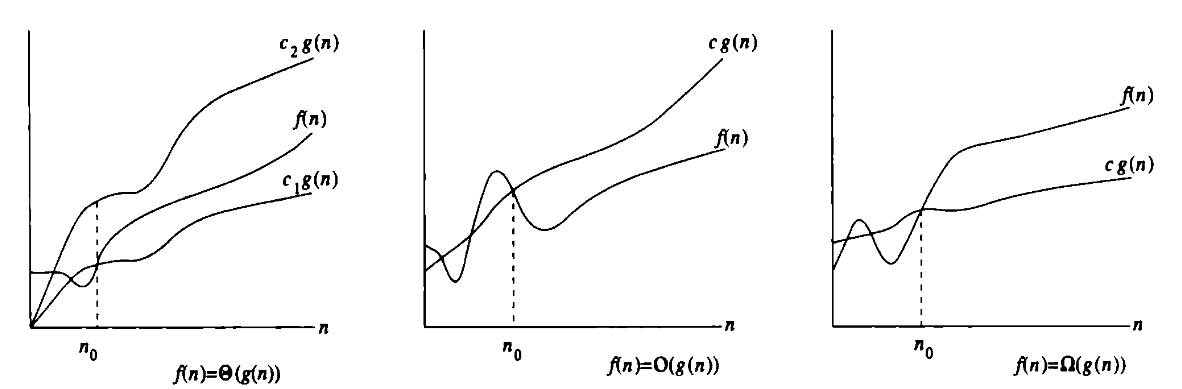
\includegraphics[width=12cm, height=3.7cm]{Term_1/Source/Pirctures/notations.png}
\end{frame}

\begin{frame}[fragile]{Рост функций}{Примеры}
\[\forall a > 0, b \in \mathbb{R}, c \in \mathbb{R}, f(n) = an^2 + bn + c  \rightarrow f(n) = \Theta(n^2)\]
\[c_1 = a / 4, c_2 = 7a/4, n_0 = 2 \cdot max(|b|/a, \sqrt{|c|/a})\]
Более того, 
\[\forall p(n) = \sum_{i=0}^{d} a_i n^i, a_d > 0 \Rightarrow p(n) = \Theta(n^d)\]
\end{frame}

\begin{frame}[fragile]{Рост функций}{Примеры}
\[f(n) = \Theta(g(n)) \Rightarrow f(n) = \mathcal{O}(g(n))\]
\[\forall f(n) = an + b, a > 0 \Rightarrow f(n) = \mathcal{O}(n^2)\]
\[c = a + |b|, n_0 = max(1, -b/a)\]
\end{frame}

\begin{frame}[fragile]{Рост функций}{Примеры}
\[\forall g(n), f(n) \rightarrow f(n) = \Theta(g(n)) \Leftrightarrow f(n) = \Omega(g(n)), f(n) = \mathcal{O}(g(n))\]
\end{frame}

\section{Двоичный поиск}
\subsection{Двоичный поиск}
\begin{frame}[fragile]{Двоичный поиск}{Задача}
Дан массив A из n элементов \[A_0, A_1, ..., A_{n-1}\] такой что: \[A_0 \leq A_1 \leq ... \leq A_{n-1}\] Дано целевое значение T. Нужно найти индекс T в A или его отсутствие.
\end{frame}

\begin{frame}[fragile]{Двоичный поиск}{Алгоритм}
\begin{lstlisting}[language=C++]
int binary_search(int* A, int n, int T) {
    int L = 0;
    int R = n - 1;
    while (L <= R) {
        int m = floor((L + R) / 2.0);
        if (A[m] < T) {
            L = m + 1;
        } else if (A[m] > T) {
            R = m - 1;
        } else {
            return m;
        }
    }
    return -1;
}
\end{lstlisting}
\end{frame}

\begin{frame}[fragile]{Двоичный поиск}{Правильный алгоритм}
\begin{lstlisting}[language=C++]
int binary_search(int* A, int n, int T) {
    int L = 0;
    int R = n - 1;
    while (L <= R) {
        int m = L + (int)floor((R - L) / 2.0);
        if (A[m] < T) {
            L = m + 1;
        } else if (A[m] > T) {
            R = m - 1;
        } else {
            return m;
        }
    }
    return -1;
}
\end{lstlisting}
\end{frame}


\appendix
\section<presentation>*{\appendixname}
\subsection<presentation>*{Useful links}

\begin{frame}[allowframebreaks]
  \frametitle<presentation>{Полезные ссылки}
    
  \begin{thebibliography}{10}
{
  \beamertemplatearticlebibitems
  
  \bibitem{broken}
  \texttt{Nearly All Binary Searches and Mergesorts are Broken}
  \newblock \href{https://ai.googleblog.com/2006/06/extra-extra-read-all-about-it-nearly.html}{\texttt{https://bit.ly/2MdGqfU}}
  
  \bibitem{Kormen1}
  \texttt{Т.Кормен, Ч.Лейзерсон, Р.Ривест, К.Штайн - Алгоритмы. Построение и анализ. Глава 3}
  \newblock \href{https://bit.ly/2wFzphU}{\texttt{https://bit.ly/2wFzphU}}

}


  \end{thebibliography}
\end{frame}

\end{document}


